\documentclass[12pt, letterpaper]{article}
\usepackage[utf8]{inputenc}
\usepackage{graphicx}
\usepackage{float}
\usepackage{color}
\usepackage{hyperref}
\hypersetup{
    colorlinks=true,
    linktoc=all,
    citecolor=blue,
    urlcolor=blue,
}
\usepackage[super]{nth}

\title{Statistical Analysis of Baseball Players}

\author{Wesley Soo-Hoo, Xander Hughes}
\date{\today}

\begin{document}

\maketitle

\begin{abstract}
In the 21st century, Major League Baseball general managers began using statistical tools to determine player value. By evaluating players by gameplay metrics instead of imprecise qualitative measures, general managers can accurately determine what players bring to a team. However, subjective factors influence the hiring process and baseball players may not yet be valued in proportion to their effect on teams. In this paper, we use Sabremetric statistics to attempt to predict player salaries and find out if they are being paid fairly.
\end{abstract}

\section{Introduction}
We will be using Principle Components Analysis (PCA) to find the most descriptive ways to categorize MLB baseball players' statistics. This technique collects a variety of data points in a many-dimensional space, and finds a new set of basis vectors which are better suited to describing the variation in the data set. This technique is used in a wide variety of applications, and so specific ethical implementations of PCA in general are difficult to itemize. However, it should be said that the mappings the algorithm finds are suited specifically to the data the algorithm has been trained on. As such, these data should be chosen carefully with sources of bias in mind and the results should be taken with a grain of salt, knowing that patterns in data can unexpectedly be confounded by existing social bias in the environment that created the data. 
\par In our investigation, we compile baseball performance statistics (as well as salaries) from a wide sample of former and current MLB players. We use PCA to find the components in 'baseball stats-space' that best describe the variation between players. We then analyze the extent to which a player's statistics can predict their salary. Using a sample of players reserved for the testing phase, we will project player data onto the stats-space's principal components, find other similar players, and observe how well we can guess the test players' salary from these data. If we predict salaries well, we will know that in-game performance is the driving factor in MLB contracts. If not, there may be non-game factors which provide insight in hiring bias.

\section{Methods}
Data was collected from the Lahman Baseball Database \cite{lahman}, which provides traditional baseball metrics dating back to 1871. To simplify the data processing, the dataset was limited to only the \nth{21} century, which provided over 3000 players from which to sample.
\par The various statistics for each player were collected into a sequence of vectors in a many-dimensional space, where each dimension represents one type of statistic. By finding the covariance matrix of the normalized vectors and taking its eigendecomposition, we obtained the principle components of variation in the player-statistic data. Because player records give the batting, fielding, and pitching scores separately (and in fact the counts of each of these records are usually different for a single player), we repeat this step individually for batting, fielding, and pitching data.
\par Next, we select the five most significant eigenvectors and project the player data onto them, forming a low-dimensional space in which players are still highly distinguishable. We then take a test set of player data (previously withheld from the eigendecomposition process) and project it onto that same space. In order to predict the salary of a player, for each point in the test set we find the 20 nearest points in player-space. The mean salary of these nearest players approximates the test player's salary. The RMS error of this approximation is recorded and used to evaluate the system. For all of the systems inputs, outputs, and error calculations, we used the base 10 log of salaries in order to account for the logarithmic distribution of contract values.

\section{Detailed Findings}

\subsection{Raw Data}
After analyzing players from 2000 to 2016, the approximation' RMS error was found. There are three values: one for the model using pitching data, one with batting data, and one with fielding data. The errors are:

\begin{enumerate}
    \item Pitching based: RMS($log_{10}$ salary) = \textbf{0.30}
    \item Batting based:  RMS($log_{10}$ salary) = \textbf{0.31}
    \item Fielding based: RMS($log_{10}$ salary) = \textbf{0.35}
\end{enumerate}

Some context for these numbers is needed: the standard deviation of the log salaries (which is equivalent to the error of approximating player salaries as the mean value) is \textbf{0.4}, meaning that our model is slightly better than guessing. 

\begin{table}
\begin{center}
\begin{tabular}{|p{2cm}||p{4cm}|p{4cm}|}
\hline
\multicolumn{3}{|c|}{Summary of Computed Eigenvectors} \\
\hline
Category & PC\#1 & PC\#2\\
\hline
\hline
Pitching & Low all except ERA, BAOpp, SV, G (0) & Low: SV, G, high: BAOpp, ERA\\
\hline
Batting & High all except SH (0) & Low: 3B, SB, CS, SH, high: HR, RBI, IBB\\
\hline
Fielding & All high & High: PB SB CS low: A DP E\\
\hline

\end{tabular}
\end{center}
\caption{Top PCA Features of Statistic Data}
\label{eigs}
\end{table}

In order to gain insight into the algorithm, we inspected the eigendecomposition results. \textbf{Table \ref{eigs}} shows the general trends of the two most significant eigenvectors in each model. We then graphed player salaries against these calculated features in order to judge patterns by eye. \textbf{Figures \ref{pitch}, \ref{bat}, \ref{field}} show the results for pitching, batting, and fielding data respectively.

\begin{figure}[H]
\centering
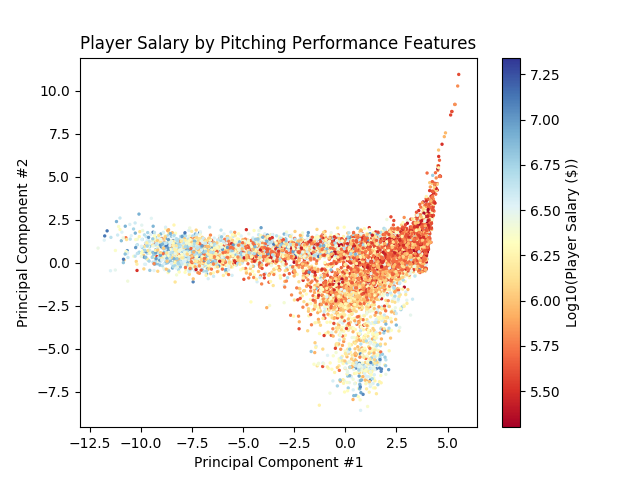
\includegraphics[scale=0.65]{pitching.png}
\caption{Pitching Results}
\label{pitch}
\end{figure}

\begin{figure}[H]
\centering
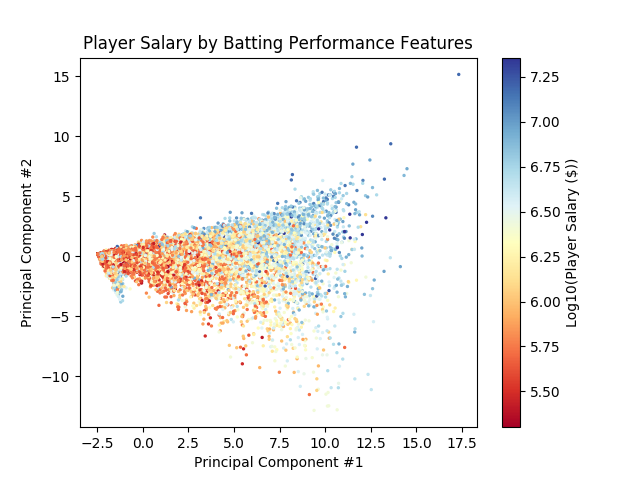
\includegraphics[scale=0.65]{batting.png}
\caption{Batting Results}
\label{bat}
\end{figure}

\begin{figure}[H]
\centering
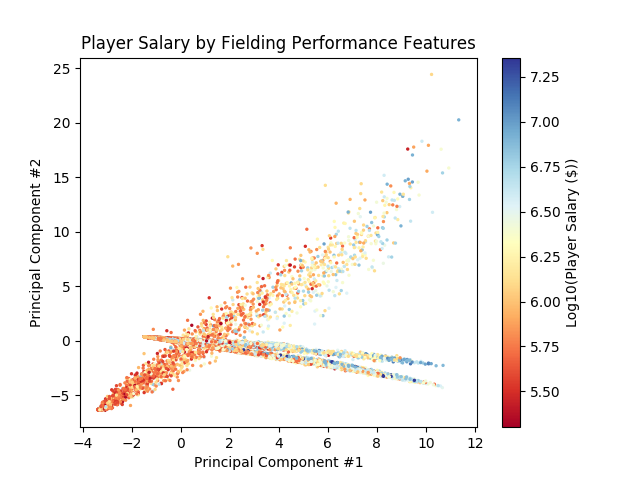
\includegraphics[scale=0.65]{fielding.png}
\caption{Fielding Results}
\label{field}
\end{figure}

\subsection{Analysis}

There is clear clustering in each of the graphs. This is an encouraging sign: with just two principal components, the highest-payed players can be reasonably distinguished from the others. Interestingly enough, these graphs also show specializations of players. For example, the bottom cluster of the pitching graph shows pitchers with low game counts and high saves. We interpret this region to consist of closers, so it seems reasonable that the most extreme of these players would be highly paid. Meanwhile, the fielders' data is very obviously divided into two groups, which we interpret to be a distinction between outfielders and infielders (since the first two principal components distinguish between putouts and assists). However, The clustering is not perfect, and in any region there exist players across the salary spectrum. There are two explanations for this, one relating to our methods and one describing the baseball industry. 

First, our data handling procedures were not optimal for classifying players. Our most important shortcoming is the fact that we analyze batting, pitching, and fielding performance separately. Therefore the salary estimator based on batting performance lacks information about the player's fielding ability, and so would estimate a high salary for a good batter even if they were an incompetent second baseman.

On the other hand, errors in our model could reflect non-performance influences on contracts. The first factor that could affect salary is fanbase bias. From a team owner's perspective, more popular players draw better ticket sales. This is one of the reasons why players such as David Price, who in 2019 was ranked as slightly above average by FanGraphs, was paid \$31 million, which was the fifth highest a pitcher has been paid \cite{baseball-reference-price}. While this does not help with gameplay, it benefits the team financially. Whether this is a net gain (Bryce Harper, Philadelphia Phillies \cite{baseball-reference-harper}), or net loss (Albert Pujols, Los Angeles Angels \cite{baseball-reference-pujols}), team management had a valid decision to offer a high contract.

Another factor that could affect salary is the macroeconomics of baseball. Players fit different archetypes, and teams have needs for players of different archetypes. Similarly to supply and demand in the market, different years have varying players on the market, which drives the contract value of players signed during that time. For example, the 2018 offseason had a notoriously weak free-agent class \cite{rosterresource-2018-fa}, which resulted in the two superstars, Bryce Harper and Manny Machado, both receiving contracts worth over \$25 million.

Given these factors, it is clear that predicting player contracts on statistics alone is implicitly inaccurate. In addition, projecting player value based on similar players' contracts in similar years is flawed, as salary does not accurately reflect player value.

\section{Recommendations}
\subsection{Takeaways}
The data show that computational analysis of player statistics reveals some trends in salaries. However, our estimations of salaries differ significantly from what players are actually paid. While there are reasons to believe that similar players are paid similarly, there are a number of external factors that can bias player salaries in either direction. An understanding of our model and the relevant external factors could help a baseball team hire more cost-effective players, and give better contracts to players who may be systematically overlooked.

\subsection{Future Work}
While the current method does not accurately predict player contract value, there are possible extensions which may improve it. The simplest and most effective way is to use the data to predict WAR (Wins Above Replacement), a modern baseball statistic that is widely accepted to approximate a player's value \cite{fangraphs-war}. Another improvement to the algorithm is to implement more modern baseball statistics. With the introduction of StatCast (a new data collection system) to the MLB, all baseball data from all games is available, from the launch velocity of a home run hit by Mike Trout \cite{baseball-savant-trout} to the spin rate of a curveball thrown by Clayton Kershaw \cite{baseball-savant-kershaw}. This data, in combination with traditional baseball metrics and sophisticated computer algorithms, can be used to better predict player value.

\bibliography{references.bib}
\bibliographystyle{IEEEtran}

\end{document}
